%
% This is where the packages are declared

\documentclass[]{article}

\usepackage[english]{babel}
\usepackage[utf8]{inputenc}
\usepackage{amsmath}
\usepackage{graphicx}
\usepackage[colorinlistoftodos]{todonotes}
\usepackage{hyperref}
\begin{document}

%
% = = = = = = = = = = = = = = = = = = = = = = = = = = = = = = = = = = = = = = = = = = = = = = = = = = = = = =
% % % % % % % % % % % % % % % % % % % % % % % % % % % % % % % % % % % % % % % % % % % % % % % % % % % % % % % 
%%%%%%%%%%%%%%%%%%%%%%%%%%%%%%%%%%%%%%%%%%%%%%%%%%%%%%%%%%%%%%%%%%%%%%%%%%%%%%%%%%%%%%%%%%%%%%%%%%%%%%%%%%%%%



%%%%%%%%%%%%%%%%%%%%%%%%%%%%%%%%%%%%%%%%%%%%%%%%%%%%%%%%%%%%%%%%%%%%%%%%%%%%%%%%%%%%%%%%%%%%%%%%%%%%%%%%%%%%%
% % % % % % % % % % % % % % % % % % % % % % % % % % % % % % % % % % % % % % % % % % % % % % % % % % % % % % % 
% = = = = = = = = = = = = = = = = = = = = = = = = = = = = = = = = = = = = = = = = = = = = = = = = = = = = = =
%
% The Title, Author Name, Date, and abstract go here

\title{Note:[Amin Jourabloo, Xiaoming Liu,
Pose-Invariant Face Alignment via CNN-Based Dense 3D Model Fitting,
International Journal of Computer, 2017]
}

\author{Mengran lin \\ \href{mailto:mengranlin@tencent.com}{mengranlin@tencent.com}}
\date{\today}
\maketitle

\begin{abstract}
First you have to upload the image file (JPEG, PNG or PDF) from your computer to 
writeLaTeX using the upload link the project menu. Then use the includegraphics command
to include it in your document. Use the figure environment and the caption command to
\end{abstract}
% Here is where your content goes.
\section{What is the problem?}

Your introduction goes here! Some examples of commonly used commands and features are listed below, to help you get started. If you have a question, please use the help menu (``?'') on the top bar to search for help or ask us a question.

\section{Why is the problem interesting?}
\label{sec:examples}

\subsection{How to Leave Comments}
Comments can be added to the margins of the document using the
\todo{Here's a comment in the margin!} todo command, as shown in the example on the right
. You can also add inline comments:
\todo[inline, color=green!40]{This is an inline comment.}
\subsection{How to Include Figures}
First you have to upload the image file (JPEG, PNG or PDF) from your computer to 
writeLaTeX using the upload link the project menu. Then use the includegraphics command
to include it in your document. Use the figure environment and the caption command to
add a number and a caption to your figure. See the code for Figure \ref{fig:frog} in this
section for an example.
\begin{figure}
\centering
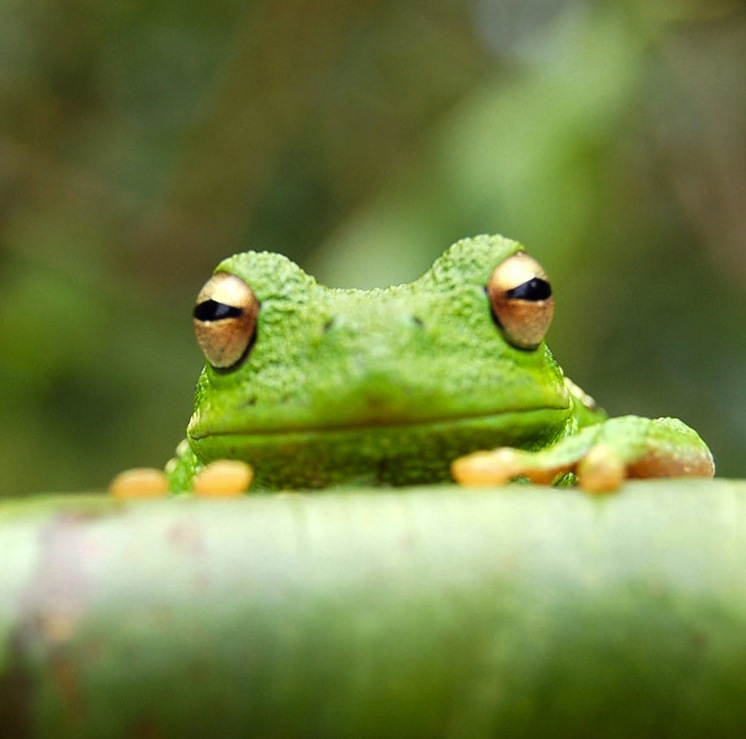
\includegraphics[width=0.3\textwidth]{./images/frog.jpg}
\caption{\label{fig:frog}This frog was uploaded to writeLaTeX via the project menu.}
\end{figure}
\subsection{How to Make Tables}
Use the table and tabular commands for basic tables --- see Table~\ref{tab:widgets},
for example.
\begin{table}
\centering
\begin{tabular}{l|r}
Item & Quantity \\\hline
Widgets & 42 \\
Gadgets & 13
\end{tabular}
\caption{\label{tab:widgets}An example table.}
\end{table}
\subsection{How to Write Mathematics}
\LaTeX{} is great at typesetting mathematics. Let $X_1, X_2, \ldots, X_n$ be a sequence of independent and identically distributed random variables with $\text{E}[X_i] = \mu$ and $\text{Var}[X_i] = \sigma^2 < \infty$, and let
$$S_n = \frac{X_1 + X_2 + \cdots + X_n}{n}
      = \frac{1}{n}\sum_{i}^{n} X_i$$
denote their mean. Then as $n$ approaches infinity, the random variables $\sqrt{n}(S_n - \mu)$ converge in distribution to a normal $\mathcal{N}(0, \sigma^2)$.

You can also create \texttt{aligned} equations as follows:
\begin{align}
&a^2 + b^2 = c^2,\\
&e^{i\theta} = \cos(\theta) + i\sin(\theta).
\end{align}

In the code, 
\begin{verbatim}
\begin{align}
&a^2 + b^2 = c^2,\\
&e^{i\theta} = \cos(\theta) + i\sin(\theta).
\end{align}
\end{verbatim}
the \texttt{\&} tells \LaTeX{} what you want to align.
\subsection{How to Make Sections and Subsections}
Use section and subsection commands to organize your document. \LaTeX{} handles all the
formatting and numbering automatically. Use ref and label commands for cross-references.
\subsection{How to Make Lists}
You can make lists with automatic numbering \dots
\begin{enumerate}
\item Like this,
\item and like this.
\end{enumerate}
\dots or bullet points \dots
\begin{itemize}
\item Like this,
\item and like this.
\end{itemize}
\dots or with words and descriptions \dots
\begin{description}
\item[Word] Definition
\item[Concept] Explanation
\item[Idea] Text
\end{description}
We hope you find write\LaTeX\ useful, and please let us know if you have any feedback
using the help menu above.
\section{Why is the problem unsolved?}
Because it is too hard.
\section{What is the authors's idea?}
assume.., He propose
\section{Inspiration or Un-trackled skills}
Inspiration
\section{Accumulation(especially the Discussion part)}
Some written better sentences.
\section{My summary(about 200 words)}
\end{document}
